\section{ANOVA}

\begin{frame}
  {Übersicht}
  \begin{itemize}[<+->]
    \item Vergleiche von Mittelwerten zwischen mehr als zwei Gruppen
    \item Mittelwertvergleiche mit mehreren Unabhängigen
    \item \alert{Warum kann man über Varianzen Mittelwerte vergleichen?}
  \end{itemize}
\end{frame}

\begin{frame}
  {Literatur}
  \begin{itemize}
    \item \citet{GravetterWallnau2007}
    \item \citet{Bortz2010}
    \item indirekt: \citet{MaxwellDelaney2004}
  \end{itemize}
\end{frame}

\subsection{Überblick}

\begin{frame}
  {Mittelwerte und Varianzen}
  \begin{itemize}[<+->]
    \item Einschränkung beim t-test: immer nur 2 Gruppen
    \item t-Test bei mehr als 2 Gruppen: komplizierte paarweise Vergleiche
      \Zeile
    \item stattdessen ANOVA: ANalysis Of VAriance
    \item Vergleich von Varianzen zwischen beliebigen Gruppen
    \item Schluss auf Mittelwerte nur indirekt über die Varianzen
      \Zeile
    \item \alert{bei zwei Gruppen: Konvergenz von t-Test und ANOVA}
  \end{itemize}
\end{frame}

\begin{frame}
  {Achtung: Gruppen vs.\ Faktoren}
  \begin{itemize}[<+->]
    \item ANOVA vergleicht immer \alert{mehrere Gruppen}
    \item Gruppen bei der einfaktoriellen ANOVA =\\
      den Ausprägungen \alert{einer unabhängigen Variable} (\zB Text-Register)
    \item diese Variablen heißen hier \alert{Faktoren}.
      \Zeile
    \item Einfluss der Faktoren auf \alert{eine abhängige} (\zB Satzlänge, Lesezeit)
      \Zeile
    \item bei mehreren Faktoren (\zB Text-Register und Jahrhundert):\\
      \alert{mehrfaktorielle ANOVA}.
  \end{itemize}
\end{frame}

\begin{frame}
  {Idee bei ANOVA (\zB drei Gruppen)}
  \begin{itemize}[<+->]
    \item \alert{H0: $\bar{x_1}=\bar{x_2}=\bar{x3}$}
    \item aber: \alert{Es gibt keinen ``Differenzwert'' für drei Mittel}\\
      (also sowas wie den t-Wert).
      \Zeile
    \item daher \alert{Varianzvergleich}
    \item \alert{F-Wert} (Verteilung unter H0 bekannt) als Test-Statistik
  \end{itemize}
  \pause
  \vspace{0.5cm}
  \begin{center}
    \alert{$F=\frac{\mathsf{Varianz\ zwischen\ Stichprobenmitteln}}{\mathsf{Varianz\ in\ den\ Stichproben}}=\frac{\mathsf{Varianz\ zwischen\ Stichprobenmitteln}}{\mathsf{Varianz\ per\ Zufall}}$}
  \end{center}
\end{frame}


\subsection{Graphische Einführung}

\begin{frame}
  {Drei Stichproben}
  $x_1=[0, 1, 3, 1, 0]$\\
  $x_2=[4, 3, 6, 3, 4]$\\
  $x_3=[1, 2, 2, 0, 0]$\\

  \vspace{-0.5cm}
  \begin{center}
    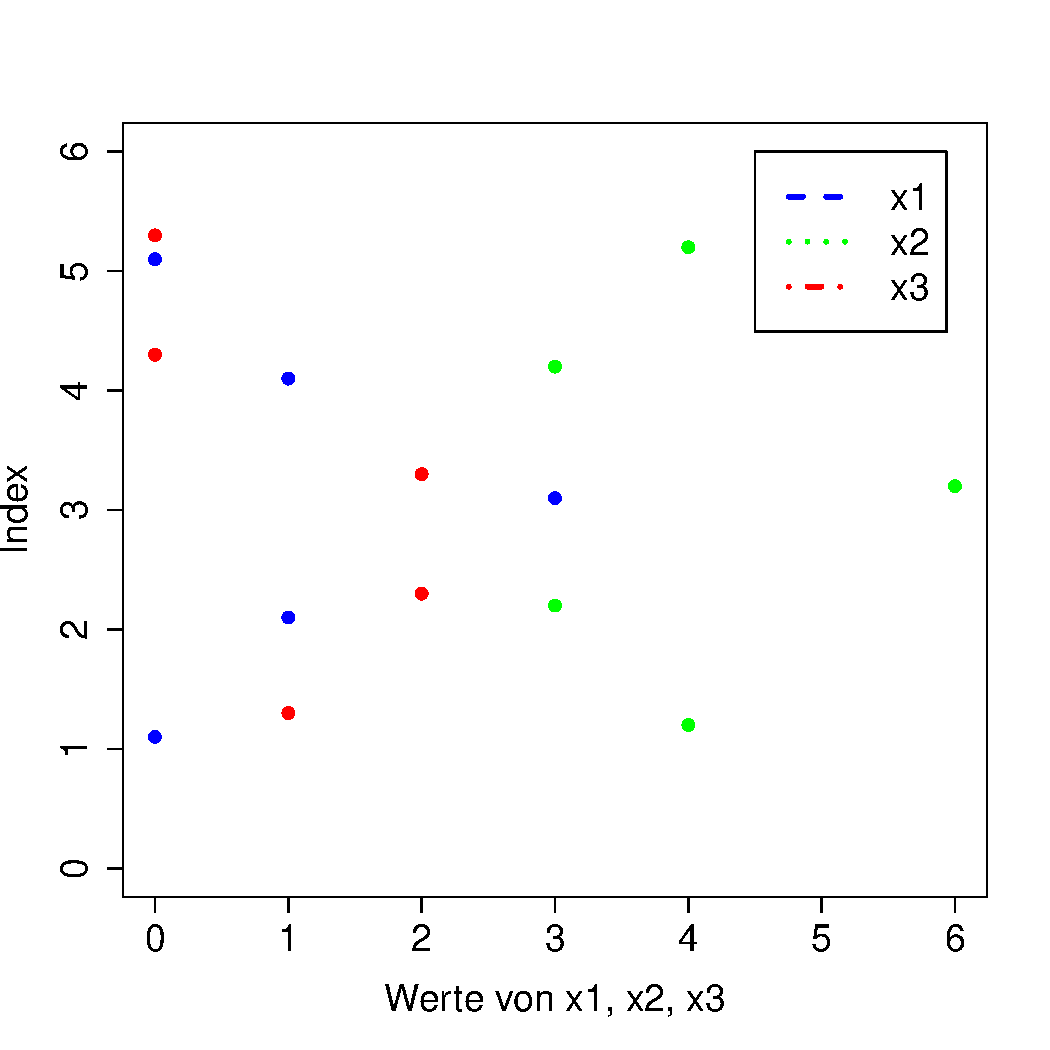
\includegraphics[width=0.45\textwidth]{graphics/anova_points}
  \end{center}
\end{frame}


\begin{frame}
  {Komponenten der Varianz von $x_1$}
  
  \begin{center}
    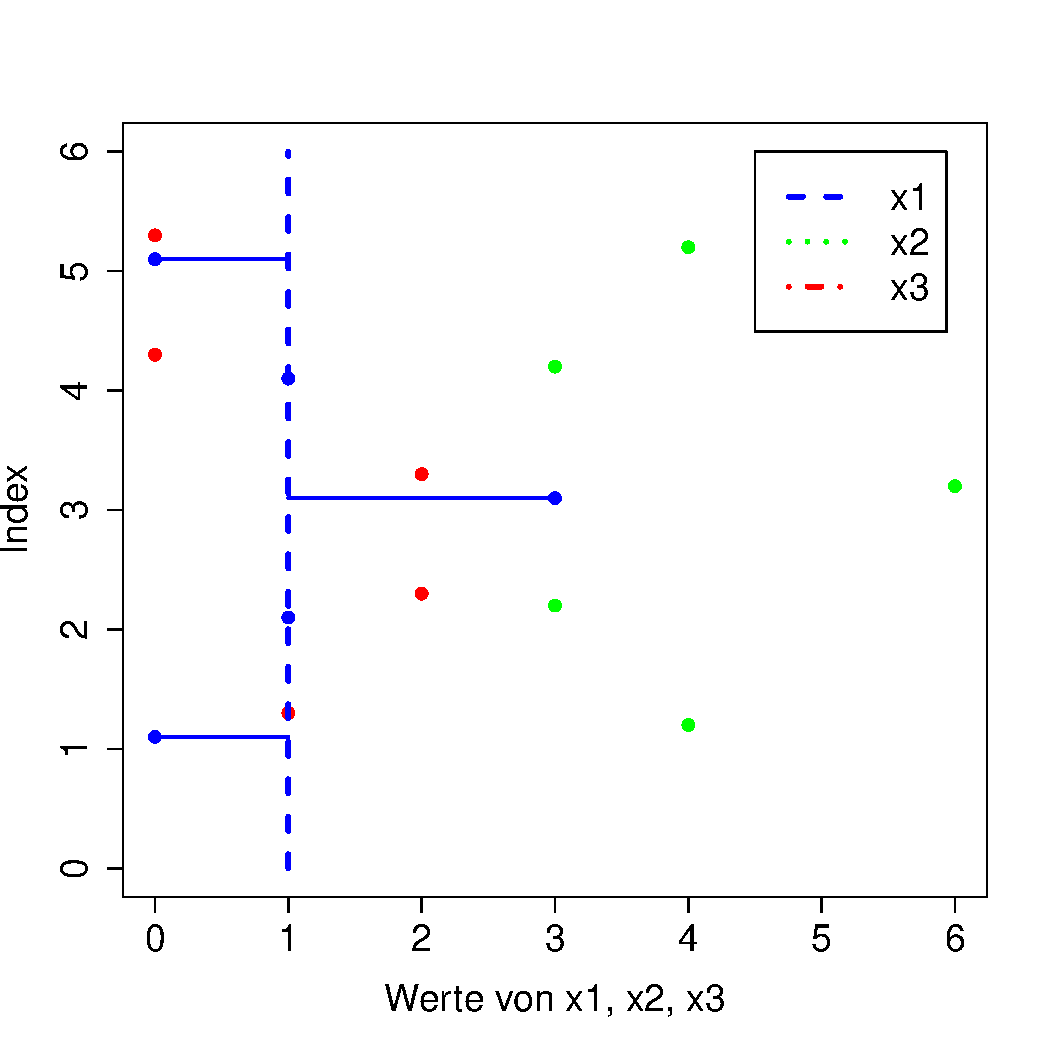
\includegraphics[width=0.45\textwidth]{graphics/anova_var_x1}\\
    $s^2(x_1)=1.5$
  \end{center}
\end{frame}

\begin{frame}
  {Komponenten der Varianz von $x_2$}
  
  \begin{center}
    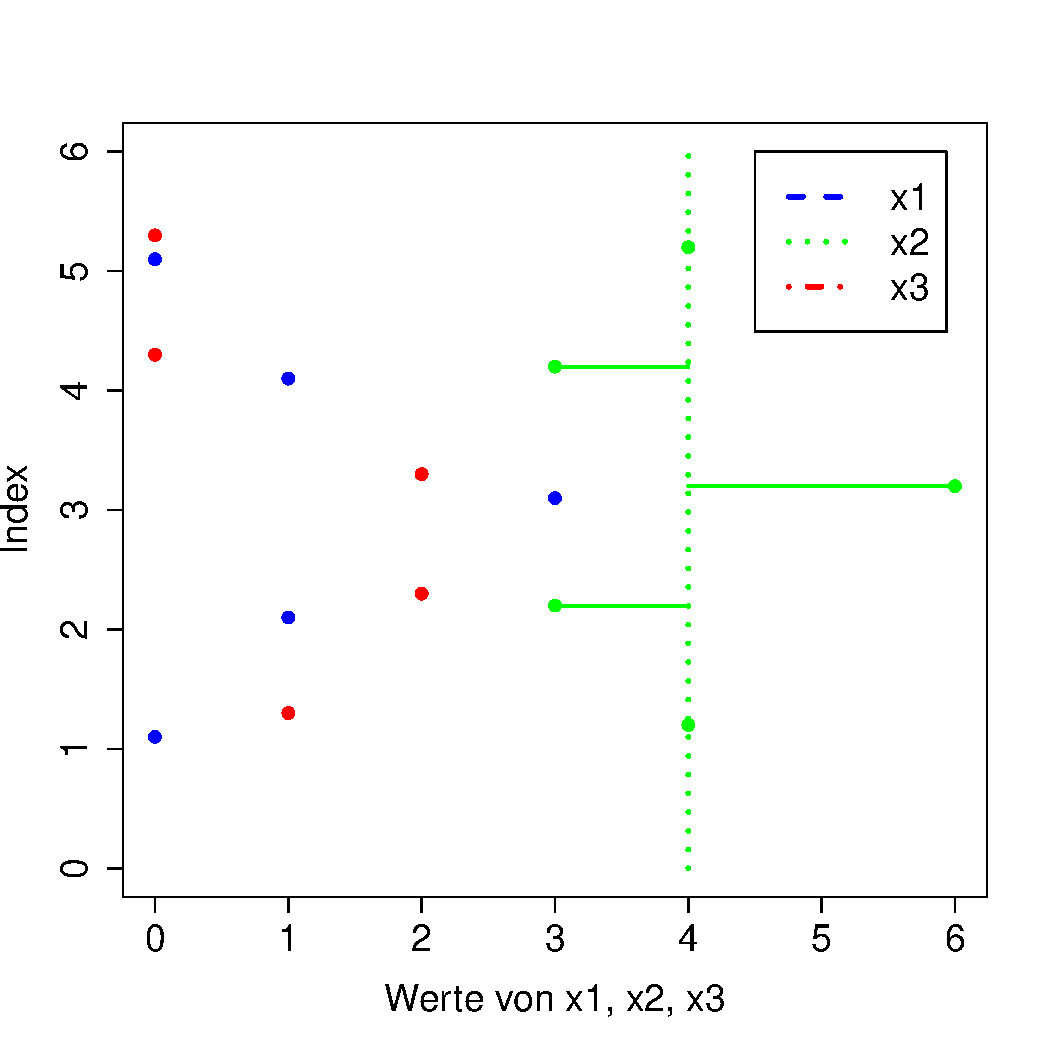
\includegraphics[width=0.45\textwidth]{graphics/anova_var_x2}\\
    $s^2(x_2)=1.5$
  \end{center}
\end{frame}

\begin{frame}
  {Komponenten der Varianz von $x_3$}
  
  \begin{center}
    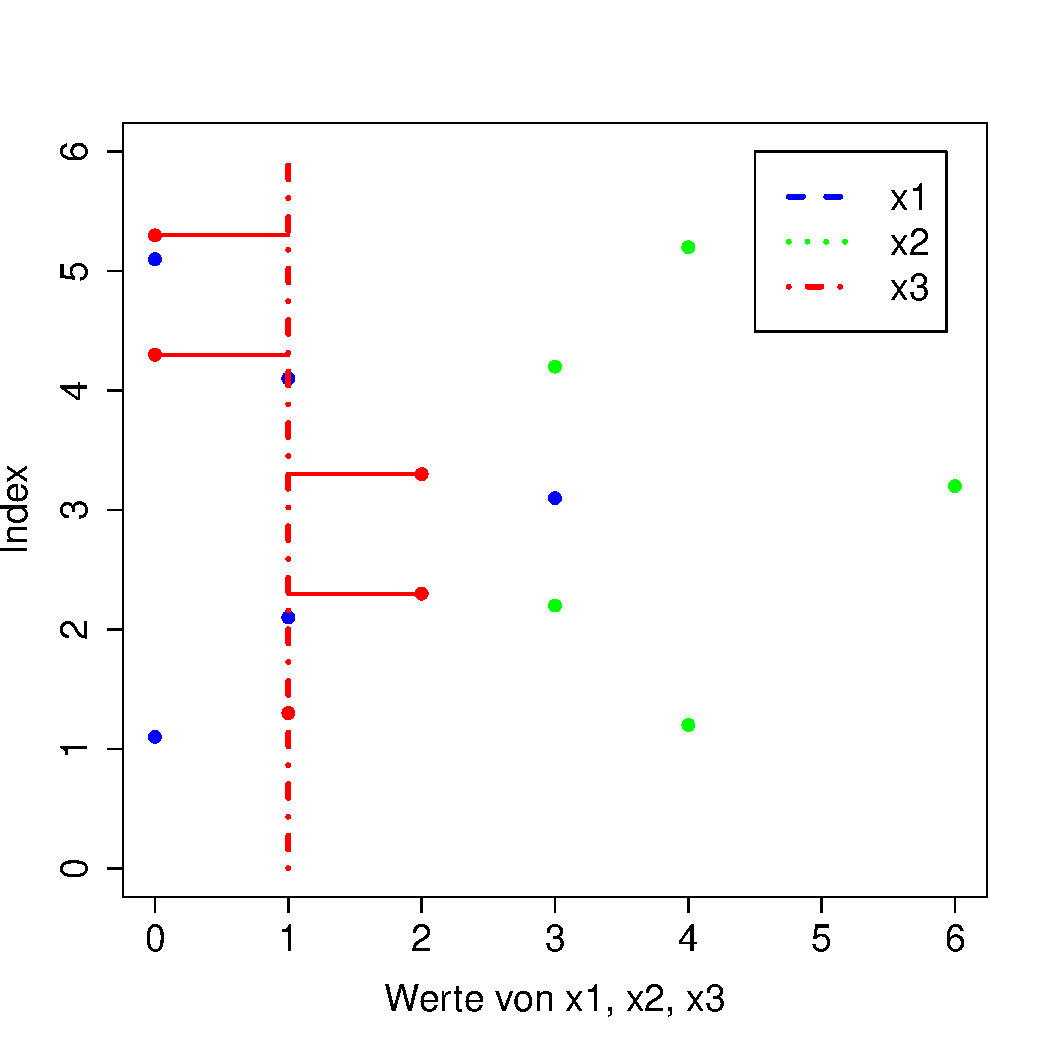
\includegraphics[width=0.45\textwidth]{graphics/anova_var_x3}\\
    $s^2(x_3)=1$
  \end{center}
\end{frame}

\begin{frame}
  {Varianz in der zusammengefassten Stichprobe $X$}
  
  \begin{center}
    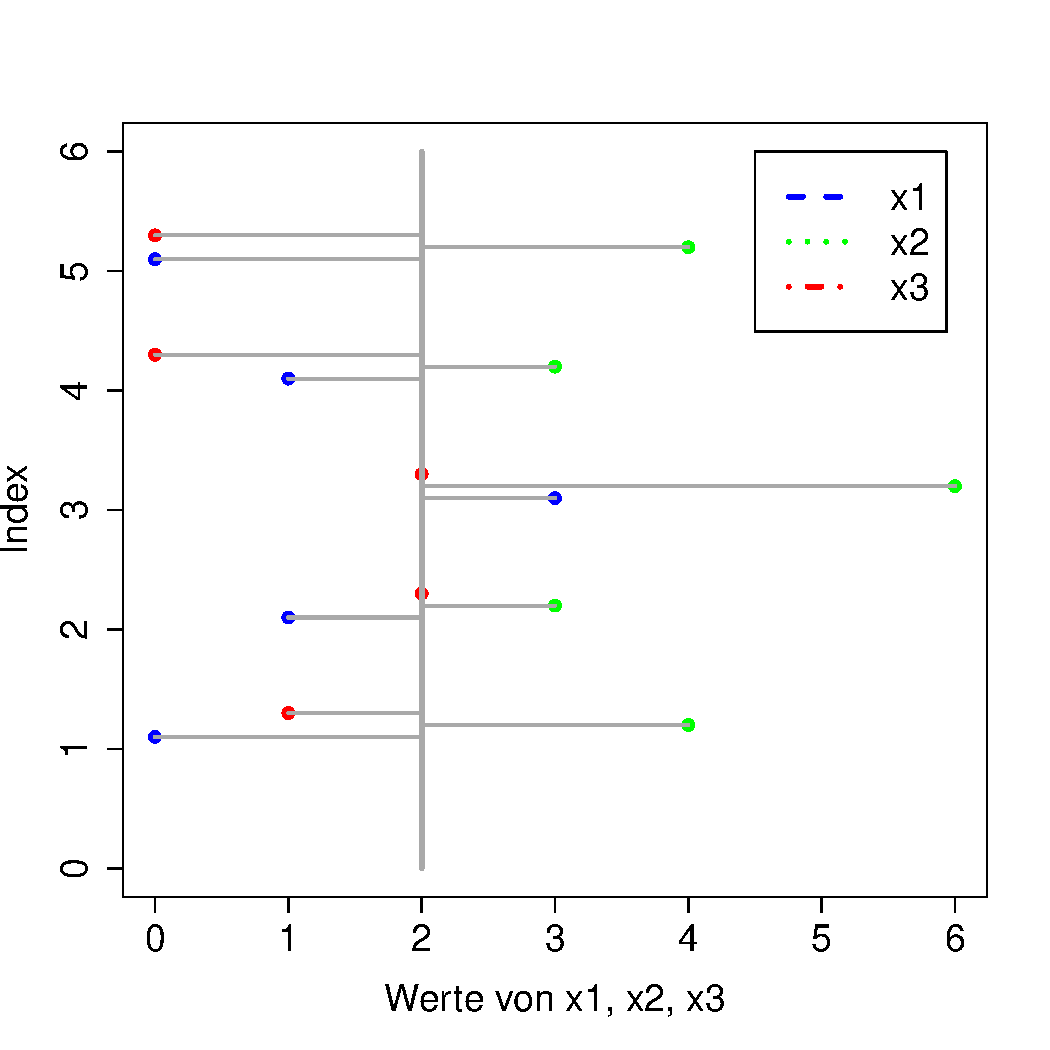
\includegraphics[width=0.45\textwidth]{graphics/anova_var_total}\\
    $s^2(X)=3.29$
  \end{center}
\end{frame}

\begin{frame}
  {Varianz zwischen den drei Gruppen}
  
  \begin{center}
    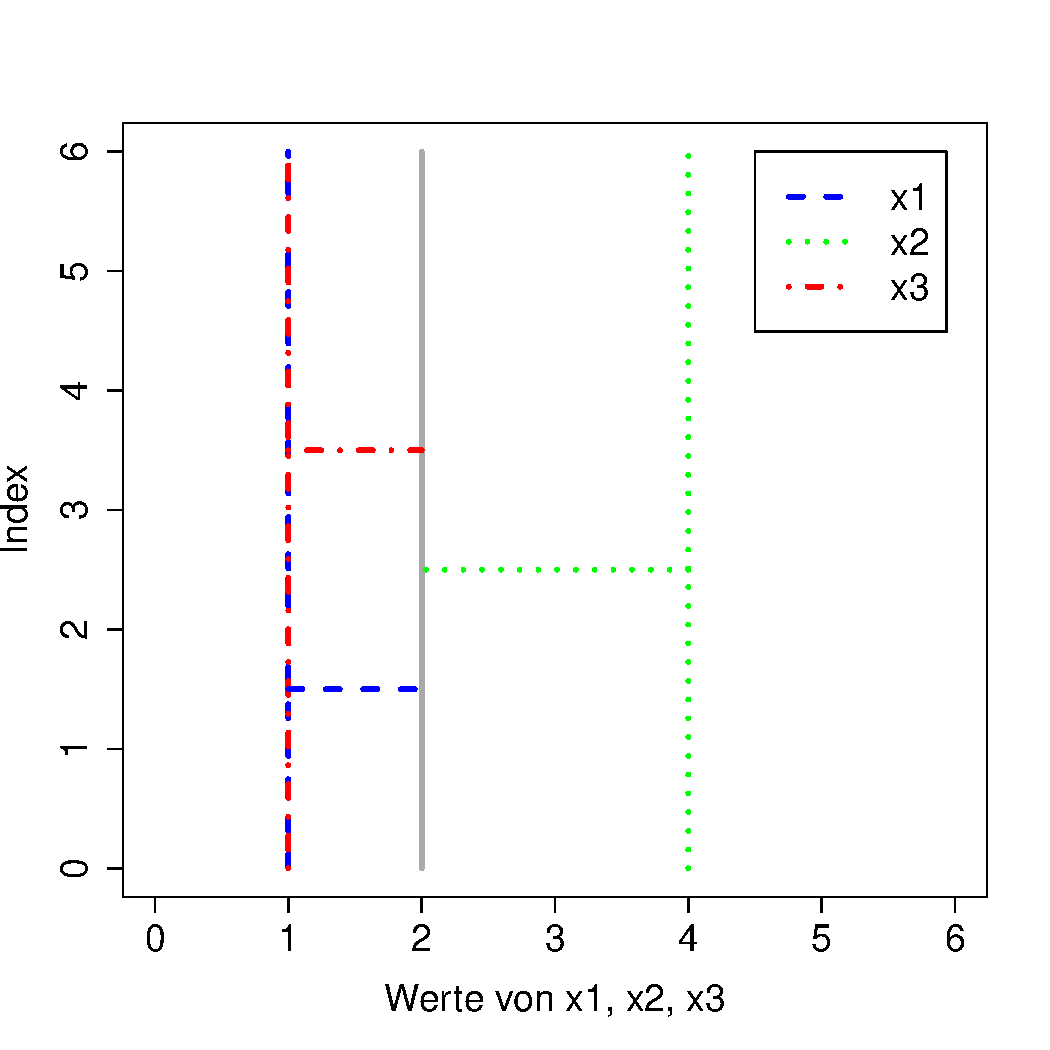
\includegraphics[width=0.45\textwidth]{graphics/anova_var_between}\\
    $s^2([\bar{x_1}, \bar{x_2}, \bar{x_3}])=1.33$\\
    \vspace{0.5cm}
    Achtung: Bei unterschiedlichen Stichprobengrößen\\
    ist das nicht ganz so einfach!
  \end{center}
\end{frame}


\begin{frame}
  {Es gilt bezüglich der Varianzen}

  \begin{center}
    \begin{tabular}[h!]{ccccc}
      \multirow{3}{*}{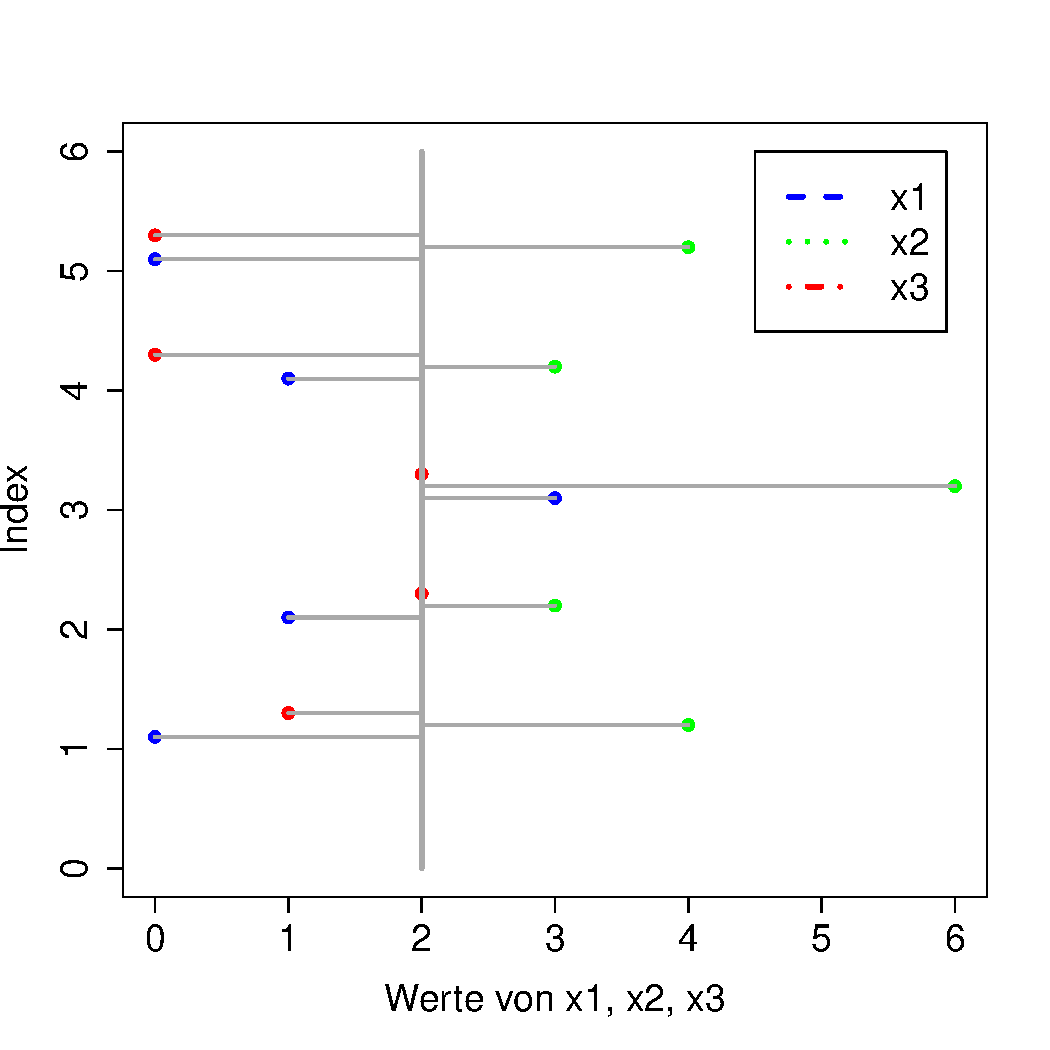
\includegraphics[width=0.2\textwidth]{graphics/anova_var_total}} & \multirow{3}{*}{$=$} & \multirow{3}{*}{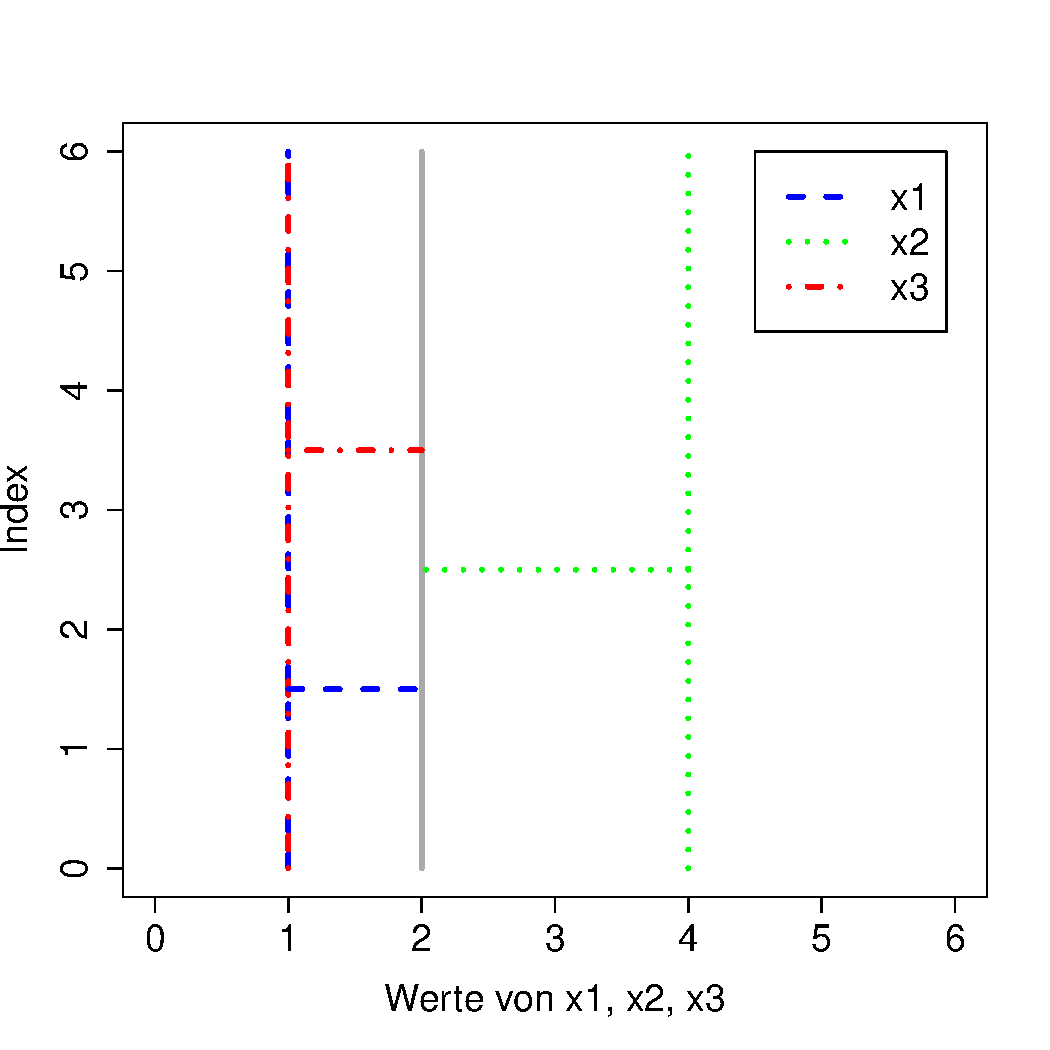
\includegraphics[width=0.2\textwidth]{graphics/anova_var_between}} & \multirow{3}{*}{$+$} & 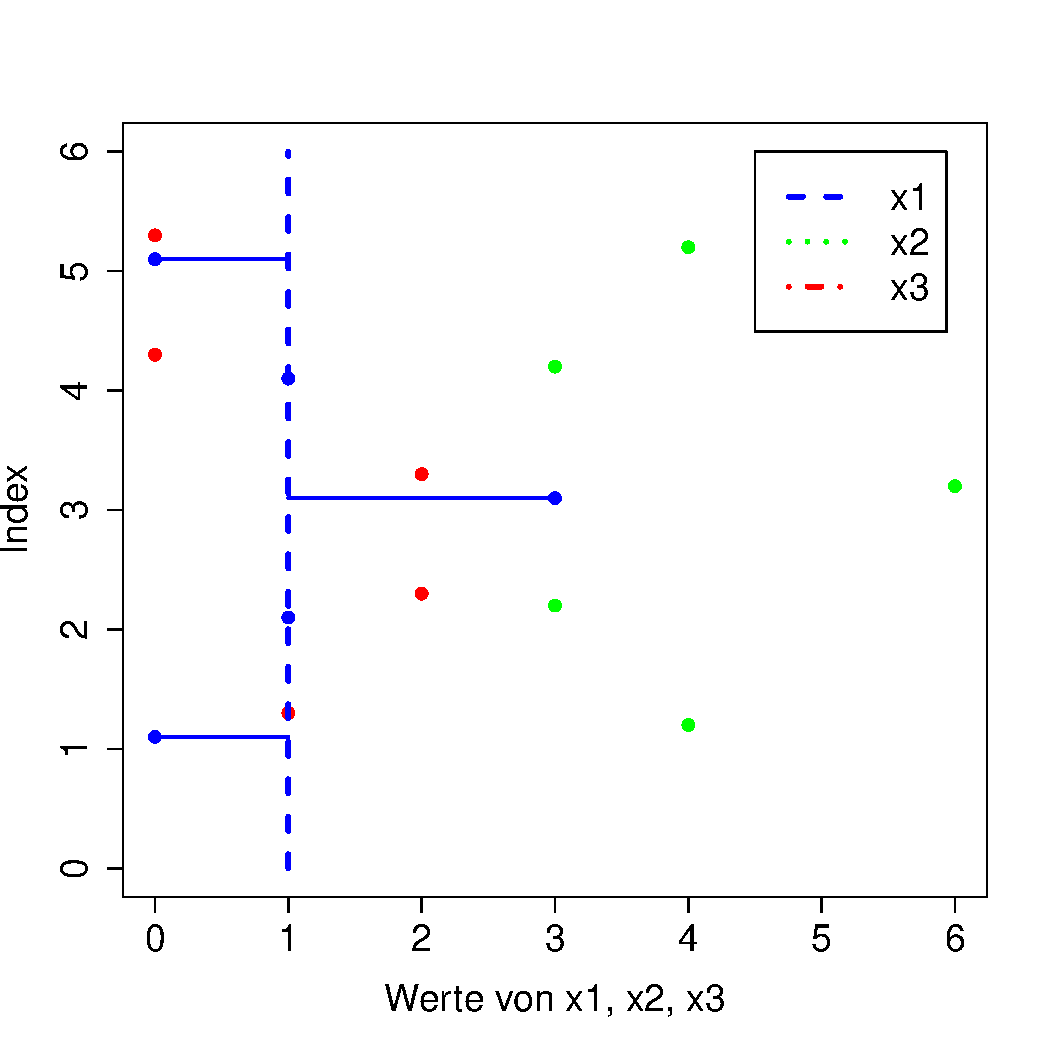
\includegraphics[width=0.15\textwidth]{graphics/anova_var_x1} \\
      &&&& 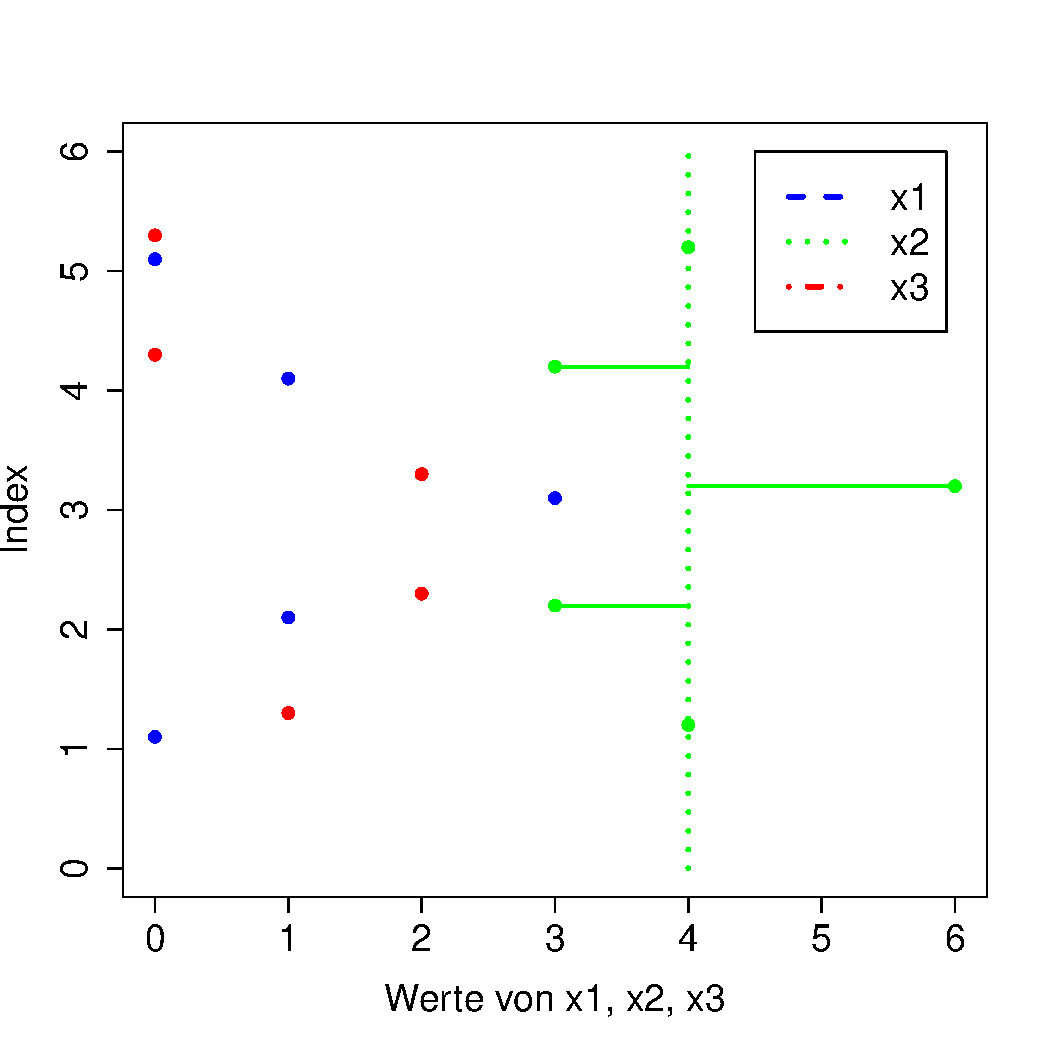
\includegraphics[width=0.15\textwidth]{graphics/anova_var_x2} \\
      &&&& 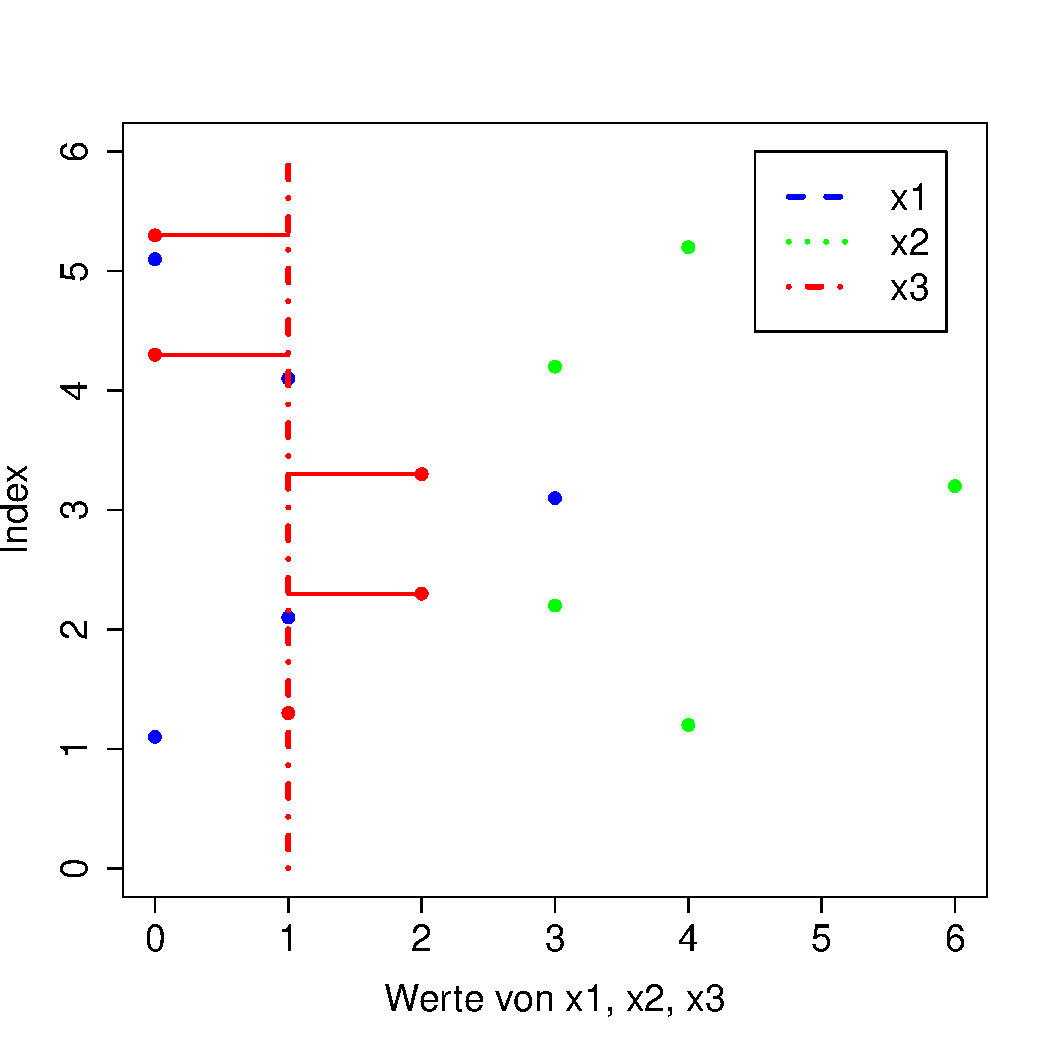
\includegraphics[width=0.15\textwidth]{graphics/anova_var_x3} \\
      \hline
      $s^2(X)$ & $=$ & $s^2(\bar{x_1},\bar{x_2},\bar{x_3})$ & $+$ & $s^2(x_1)+s^2(x_2)+s^2(x_3)$ \\
    \end{tabular}\\
    \Zeile
    \rot{Wenn man den Abstand zwischen den Mitteln verschiebt,\\\textbf{muss} die Gesamtvarianz größer werden!}
  \end{center}
\end{frame}

\begin{frame}
  {Graphische Verdeutlichung des F-Werts}
  
  \begin{center}
    \alert{$F=\frac{\mathsf{Varianz\ zwischen\ Stichprobenmitteln}}{\mathsf{Varianz\ in\ den\ Stichproben}}=\frac{\mathsf{Varianz\ zwischen\ Stichprobenmitteln}}{\mathsf{Varianz\ per\ Zufall}}$}\\
    \begin{tabular}[h!]{cc}
      \multirow{2}{*}{$F=$} & 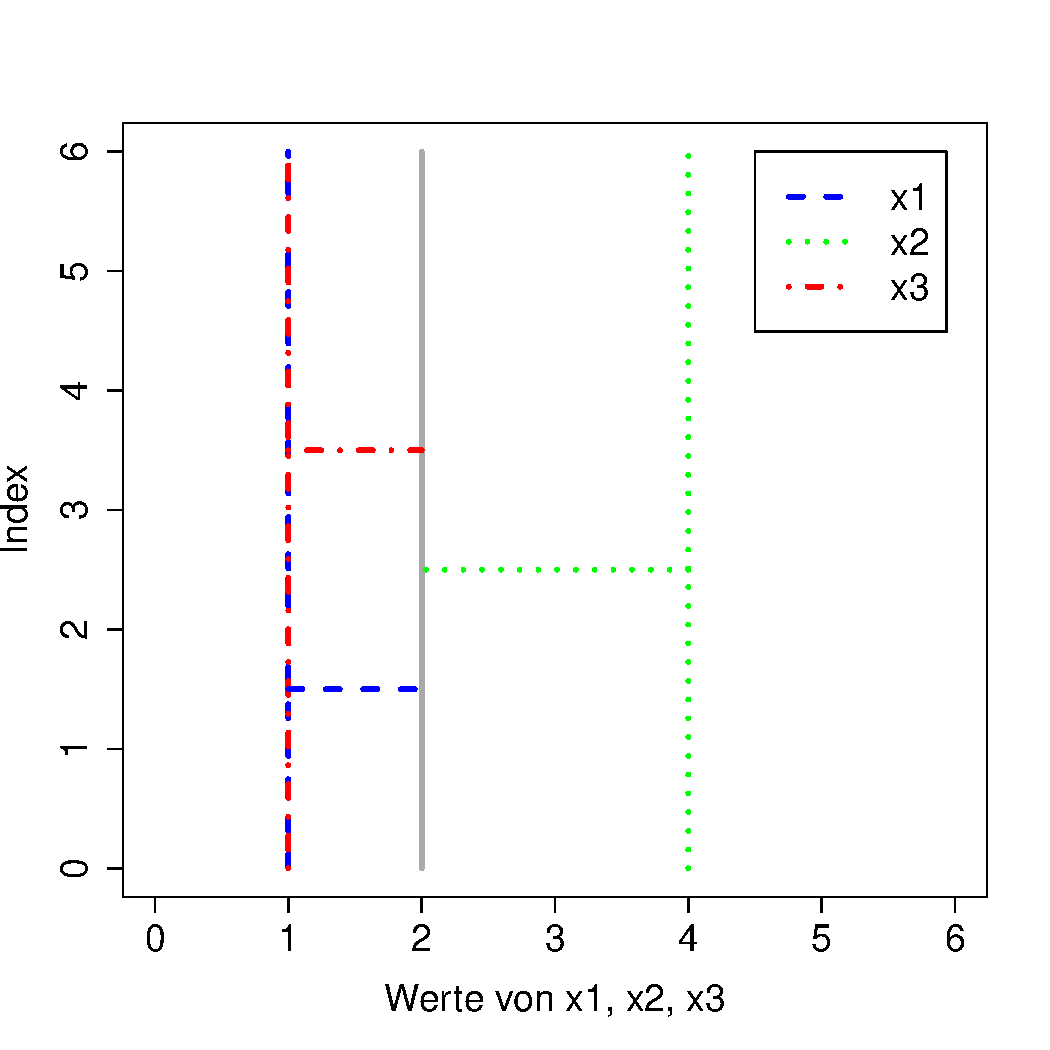
\includegraphics[width=0.2\textwidth]{graphics/anova_var_between} \\\cline{2-2}
      & 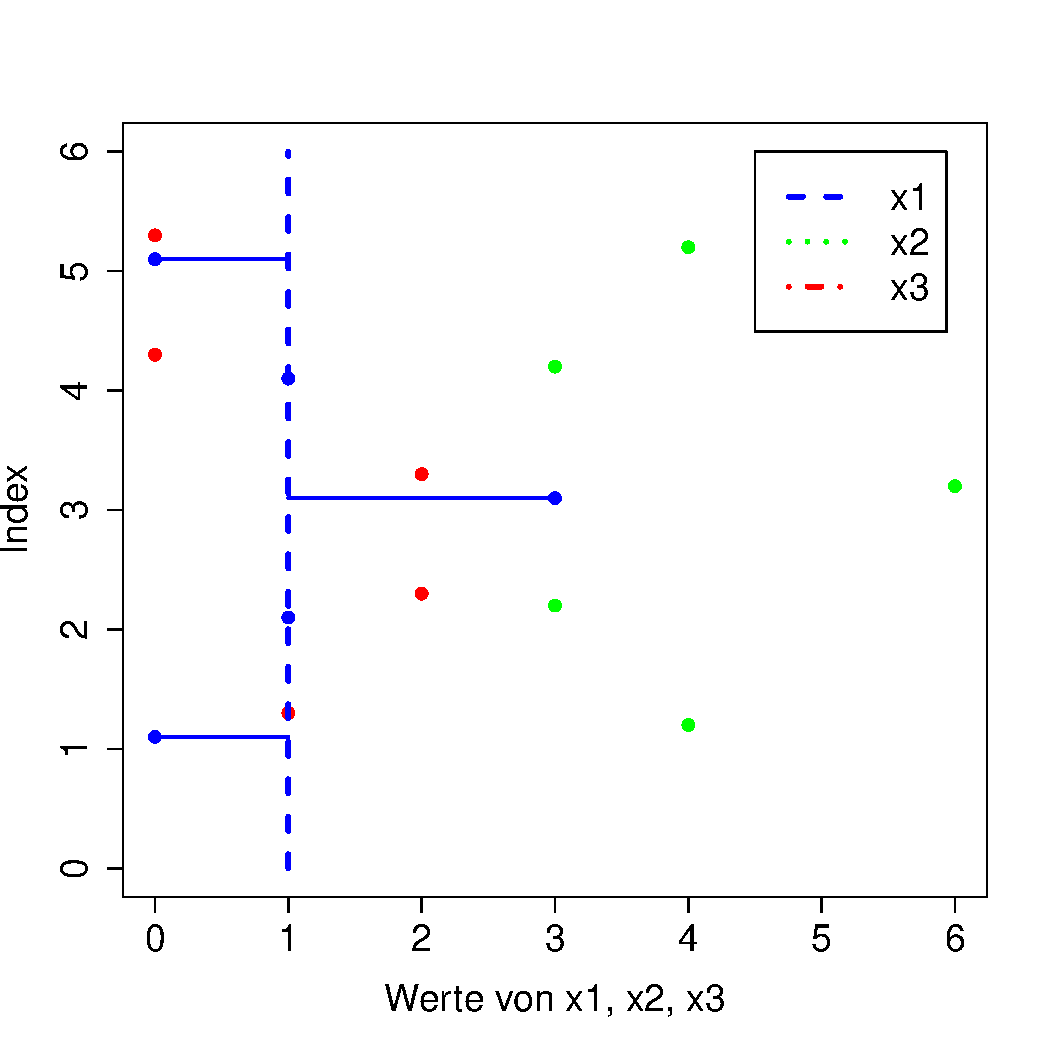
\includegraphics[width=0.2\textwidth]{graphics/anova_var_x1}\ \raisebox{1.25cm}{+}\ 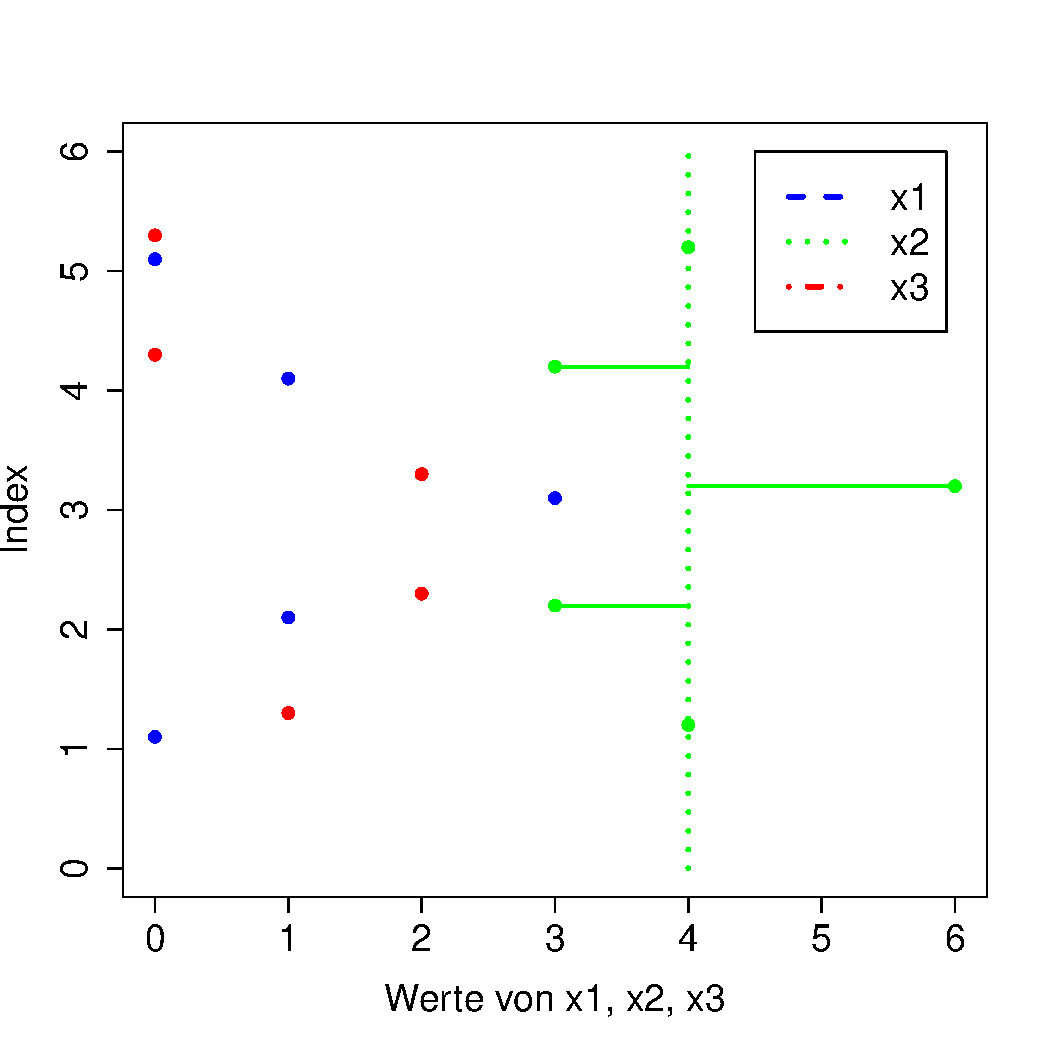
\includegraphics[width=0.2\textwidth]{graphics/anova_var_x2}\ \raisebox{1.25cm}{+}\ 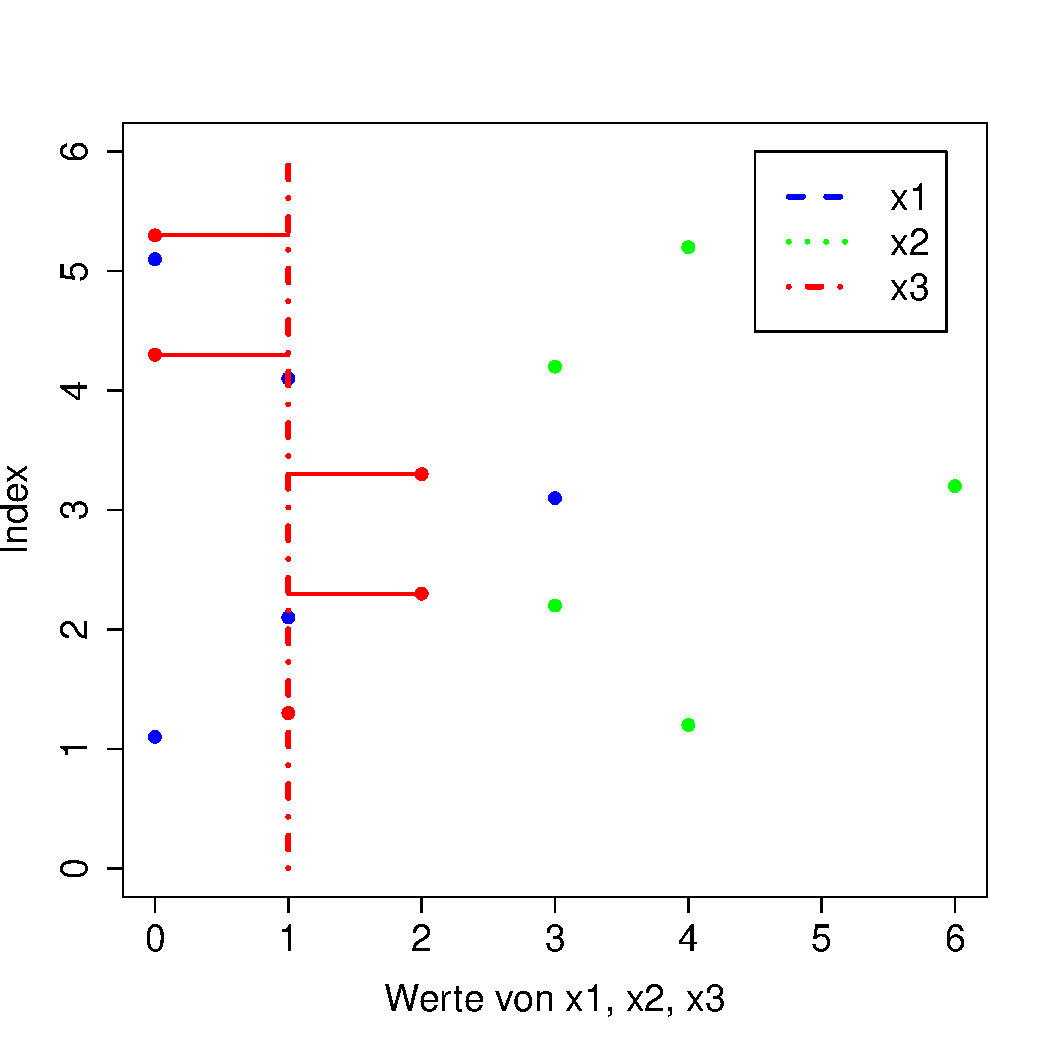
\includegraphics[width=0.2\textwidth]{graphics/anova_var_x3} \\
    \end{tabular}\\
    \Zeile
    \rot{Wenn man den Abstand zwischen den Mitteln verschiebt,\\\textbf{muss} die Gesamtvarianz größer werden!}
  \end{center}
\end{frame}

\subsection{Einfaktorielle ANOVA}

\begin{frame}
  {Wie funktioniert der F-Wert}
  \begin{itemize}[<+->]
    \item $F=\frac{\mathsf{Varianz\ zwischen\ Stichprobenmitteln}}{\mathsf{Varianz\ in\ den\ Stichproben}}$
    \Zeile
    \item Warum?
    \item $F=\frac{\mathsf{\alert{Unterschied\ durch\ Effekt}+Unterschiede\ durch\ restliche\ Varianz}}{\mathsf{Unterschied\ durch\ restliche\ Varianz}}$
    \Zeile
    \item Unter Annahme der H0 gibt es keinen Effekt, \ldots
    \item also \alert{$Unterschied\ durch\ Effekt=0$}
    \Zeile
    \item dann: $F=\frac{\mathsf{\alert{0}+Unterschiede\ durch\ restliche\ Varianz}}{\mathsf{Unterschied\ durch\ restliche\ Varianz}}=\alert{1}$
  \end{itemize}
\end{frame}

\begin{frame}
  {Notation, fast wie in Gravetter \& Wallnau, Kap.~13}
  \begin{itemize}[<+->]
    \item Anzahl der Gruppen \alert{$x_i$}: \alert{$k$}
    \item Größe der Gruppen: \alert{$n_i$}
    \item Größe der Gesamtstichprobe \alert{$X$}: \alert{$N$}
    \item Summen der Gruppen: \alert{$T_i$}
    \item Gesamtsumme: \alert{$G$}
    \item Mittel (anders als G\&W): \alert{$\bar{x_i}$}, \alert{$\bar{X}$}
    \item Summe der Quadrate (=Zähler der Varianz): \alert{$SQ(x_i)$}, \alert{$SQ(X)$}
  \end{itemize}
  \pause
  \vspace{0.5cm}
  Zur Erinnerung: $s^2(x)=\frac{\sum (x-\bar{x})}{n-1}=\frac{SQ(x)}{df(x)}$\\
\end{frame}

\begin{frame}
  {Varianz ist Varianz beim F-Wert}
  \begin{center}
    $F=\frac{Varianz\ zwischen\ den\ Gruppen}{Varianz\ in\ den\ Gruppen}=\frac{\ \ \ s^2_{zwischen}\ \ \ }{s^2_{in}}=\alert{\frac{\ \ \ \frac{SQ_{zwischen}}{df_{zwischen}}\ \ \ }{\frac{SQ_{in}}{df_{in}}}}$\\
    \vspace{0.5cm}

    denn\\
    \vspace{0.5cm}

    $s^2(x)=\frac{SQ(x)}{df(x)}$
  \end{center}
\end{frame}

\begin{frame}
  {Berechnung der SQ}
  Am einfachsten unter Beachtung von:\\
  \alert{$SQ_{gesamt}=SQ_{zwischen}+SQ_{in}$}\\

  \vspace{0.5cm}
  \pause
  Es gilt: \alert{$SQ_{gesamt}=SQ(X)=\sum(X-\bar{X})$}\\
  
  \vspace{0.5cm}
  \pause
  Außerdem: \alert{$SQ_{in}=\sum SQ(x_i)$}\\
  
  \vspace{0.5cm}
  \pause
  Damit: \alert{$SQ_{zwischen}=SQ_{gesamt}-SQ_{in}$}\\
\end{frame}

\begin{frame}
  {$SQ_{zwischen}$}
  $SQ_{zwischen}$ kann man auch direkt ausrechnen:

  \vspace{0.5cm}
  \begin{center}
    $SQ_{zwischen}=\sum\limits_i(\frac{T_i^2}{n_i})-\frac{G^2}{N}$
  \end{center}
\end{frame}


\begin{frame}
  {Aufgabe}
  $x_1=[0, 1, 3, 1, 0]$\\
  $x_2=[4, 3, 6, 3, 4]$\\
  $x_3=[1, 2, 2, 0, 0]$\\

  \begin{center}
    Bitte alle $SQ$ ausrechnen, inkl.\ $SQ_{zwischen}$ direkt.
  \end{center}

  \vspace{0.5cm}
  \scriptsize
  Tipp: Sie brauchen als Vorwissen \alert{nur}\\
  den Stoff der ersten Statistik-Sitzung:
  \begin{itemize}
    \item arithmetisches Mittel
    \item SQ
  \end{itemize}
\end{frame}

\begin{frame}
  {Freiheitsgrade ausrechnen}
  Es gilt auch hier, ähnlich wie bei den $SQ$:\\
  \alert{$df_{gesamt}=df_{zwischen}+df_{in}$}

  \vspace{0.5cm}
  $df_{gesamt}=N-1$\\[2ex]
  $df_{zwischen}=k-1$\\[2ex]
  $df_{in}=\sum\limits_{i=1}^{k}(n_i-1)=(N-1)-(k-1)$
\end{frame}

\begin{frame}
  {Alles zusammen: F-Wert}
  \begin{center}
    $F=\frac{s^2_{zwischen}}{s^2_{in}}=\frac{\ \ \ \frac{SQ_{zwischen}}{df_{zwischen}}\ \ \ }{\frac{SQ_{in}}{df_{in}}}$\\
  \end{center}

  \vspace{0.5cm}
  \begin{center}
    Bitte ausrechnen für o.\,g.\ Beispiel.
  \end{center}
\end{frame}

\begin{frame}
  {Ermitteln der kritischen Werte}
  \begin{center}
    F-Verteilung:\\
    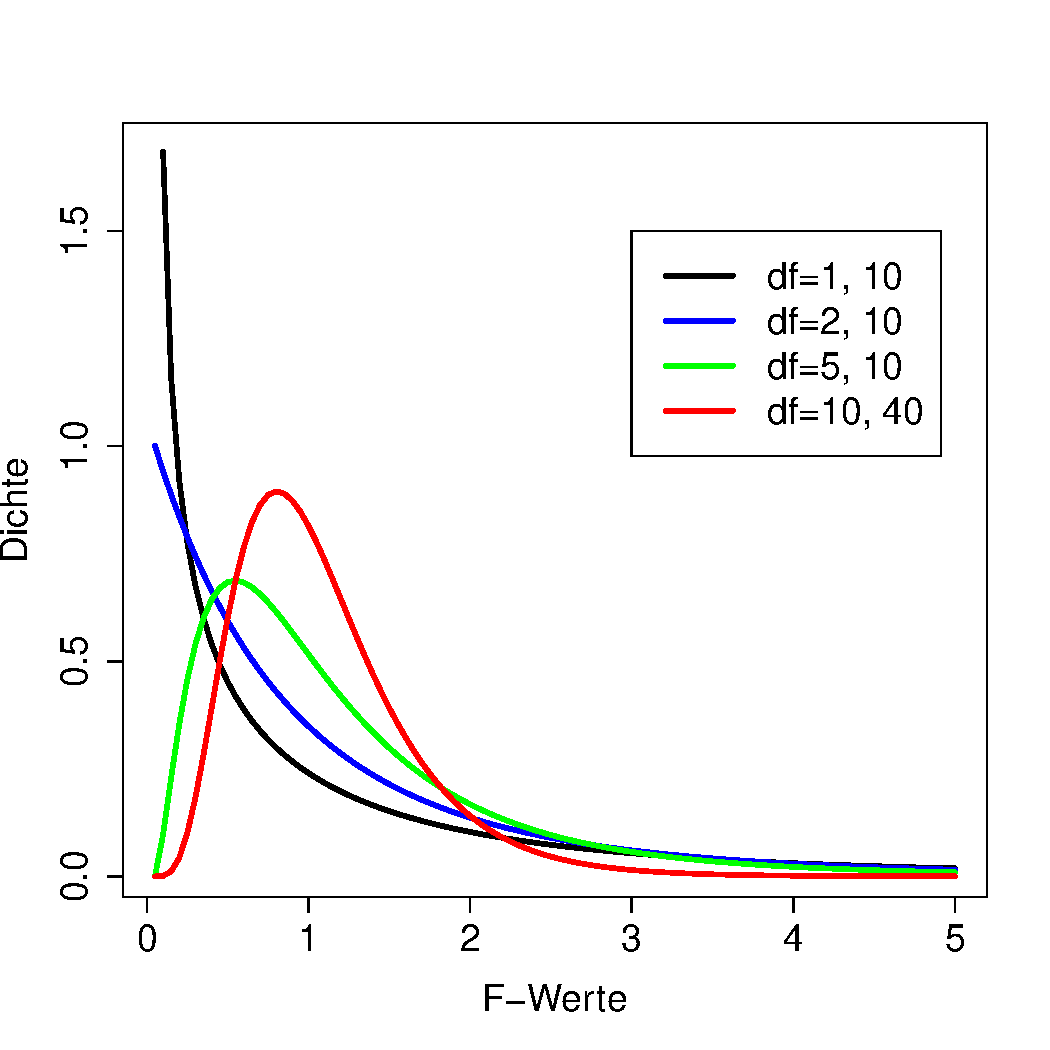
\includegraphics[width=0.3\textwidth]{graphics/anova_fdist}
  \end{center}

  \vspace{0.5cm}
  In \texttt{R} für $df_{zwischen}=2$ und $df_{in}=12$ bei sig=0.05:\\
  \texttt{> qf(0.95, 2, 12) $\Rightarrow$ 3.885294}
\end{frame}

\begin{frame}
  {Effektstärke}

  \begin{center}
    \alert{$\eta^2=\frac{SQ_{zwischen}}{SQ_{gesamt}}$}\\[4ex]
    (wieder ein $r^2$-Maß)
  \end{center}
\end{frame}

\begin{frame}
  {Post-Hoc-Tests}
  \begin{itemize}[<+->]
    \item Problem: \alert{Welche Gruppen unterscheiden sich denn nun?}
    \Zeile
    \item Lösung: Post(-Hoc)-Tests, \zB Scheff\'e-Test:
      \begin{itemize}
	\item \alert{paarweise ANOVA}
	\item aber: \alert{$k$} wird gesetzt \alert{wie bei ursprünglicher ANOVA}
	\item dadurch Vermeidung kumulierten Alpha-Fehlers\\
	  (Vorteil ggü.\ paarweisen t-Tests)
	\item weiterer Vorteil: paarweise Post-Tests nur erforderlich,\\
	  wenn \alert{Omnibus-ANOVA} bereits Signifikanz gezeigt hat
	\item und: Generalisierbarkeit zu mehrfaktorieller ANOVA\\
	  (geht mi t-Test nicht)
      \end{itemize}
  \end{itemize}

  \vspace{0.2cm}
  \pause
  \begin{center}
    Bitte ausrechnen für die oben gerechnete ANOVA.
  \end{center}
\end{frame}

\subsection{Zweifaktorielle ANOVA}

\begin{frame}
  {Wozu mehrfaktorielle Designs}

  Oft vermutet man den Einfluss \alert{mehrerer Unabhängiger} auf eine Abhängige.\\
  Beispiel: Satzlängen

  \begin{center}
    \begin{tabular}[h!]{|cc|ccc|}
      \cline{3-5}
      \multicolumn{2}{c|}{} & \multicolumn{3}{c|}{\textbf{Textsorte}} \\
      \multicolumn{2}{c|}{} & \textbf{Fiktion} & \textbf{Zeitung} & \textbf{Wissenschaft} \\
      \hline
      \multirow{2}{*}{\textbf{Jahrhundert}} & \textbf{19} & $x_{11}$ & $x_{12}$ & $x_{13}$ \\
      & \textbf{20} & $x_{21}$ & $x_{22}$ & $x_{23}$ \\
      \hline
    \end{tabular}\\
    \vspace{0.5cm}

    Hier also: $2\cdot3=6$ Gruppen
  \end{center}
\end{frame}

\begin{frame}
  {Ablauf der zweifaktoriellen ANOVA}
  \begin{enumerate}[<+->]
    \item erste ANOVA zwischen Zeilen
    \item zweite ANOVA zwischen Spalten
    \item dritte ANOVA für \alert{Interaktionen} zwischen Zeilen und Spalten
    \Zeile
    \item Interaktion: Ungleichverteilung in Gruppen, die nicht\\
      durch die Spalten- und Zeileneffekte erklärt werden kann
    \Zeile
    \item Alle drei ANOVAs sind \alert{unabhängig} voneinander!
  \end{enumerate}
\end{frame}

\begin{frame}
  {Komponenten der zweifaktoriellen ANOVA}
  \begin{itemize}[<+->]
    \item \alert{Gesamtvarianz} = Varianz zwischen Gruppen + Varianz in den Gruppen
    \Zeile
    \item \alert{Varianz zwischen den Gruppen} =\\
      Haupt-Faktoren-Varianz + \alert{Interaktions-Varianz}
    \Zeile
    \item \alert{Haupt-Faktoren-Varianz} =\\
      Varianz zwischen Faktor A-Gruppen +\\
      Varianz zwischen Faktor B-Gruppen
  \end{itemize}
\end{frame}

\begin{frame}
  {Schritt 1(1): SQ\slash df zwischen den Gruppen}
  \alert{Jede Zelle} der Tabelle ist eine Gruppe.

  \begin{center}
    \alert{$SQ_{zwischen}=\sum\limits_i(\frac{T_i^2}{n_i})-\frac{G^2}{N}$}\\

    \alert{$df_{zwischen}=k-1$} (k = Anzahl der Zellen\slash Gruppen)
  \end{center}
  \vspace{1cm}
  Beachte: \alert{Keine} Änderung verglichen mit einfaktorieller ANOVA!
\end{frame}

\begin{frame}
  {Schritt 1(2): SQ\slash df in den Gruppen}
  \alert{Jede Zelle} der Tabelle ist eine Gruppe.

  \begin{center}
    \alert{$SQ_{in}=\sum SQ(x_i)$}\\

    \alert{$df_{in}=\sum df(x_i)$}
  \end{center}
  \vspace{1cm}
  Beachte: \alert{Keine} Änderung verglichen mit einfaktorieller ANOVA!
\end{frame}

\begin{frame}
  {Schritt 2(2): SQ\slash df für Gruppe A}

  Berechnung nach dem Schema für Zwischen-Gruppen-Varianz

  \begin{center}
    \begin{tabular}[h!]{|cc|ccc||c|}
      \cline{3-5}
      \multicolumn{2}{c|}{} & \multicolumn{3}{c||}{\textbf{Textsorte}} & \multicolumn{1}{c}{}\\
      \multicolumn{2}{c|}{} & \textbf{Fiktion} & \textbf{Zeitung} & \textbf{Wissenschaft} & \multicolumn{1}{c}{}\\
      \hline
      \multirow{2}{*}{\textbf{Jahrhundert}} & \textbf{19} & $x_{11}$ & $x_{12}$ & $x_{13}$ & \alert{$A_1$}\\
      & \textbf{20} & $x_{21}$ & $x_{22}$ & $x_{23}$ & \alert{$A_2$}\\
      \hline
    \end{tabular}\\
    \vspace{0.5cm}

    Auch hier keine wesentliche Änderung:\\
    \alert{$SQ_{A}=\sum\limits_i(\frac{T_{A_i}^2}{n_{A_i}})-\frac{G^2}{N}$}\\
    \alert{$df_{A}=k_A-1$} ($k_A$ = Anzahl der \alert{Zeilen})
  \end{center}
\end{frame}

\begin{frame}
  {Schritt 2(2): SQ\slash df für Gruppe A}

  Berechnung nach dem Schema für Zwischen-Gruppen-Varianz

  \begin{center}
    \begin{tabular}[h!]{|cc|ccc|}
      \cline{3-5}
      \multicolumn{2}{c|}{} & \multicolumn{3}{c|}{\textbf{Textsorte}} \\
      \multicolumn{2}{c|}{} & \textbf{Fiktion} & \textbf{Zeitung} & \textbf{Wissenschaft} \\
      \hline
      \multirow{2}{*}{\textbf{Jahrhundert}} & \textbf{19} & $x_{11}$ & $x_{21}$ & $x_{31}$ \\
      & \textbf{20} & $x_{12}$ & $x_{22}$ & $x_{32}$ \\
      \hline\hline
      \multicolumn{2}{c|}{} & \alert{$B_1$} & \alert{$B_2$} & \alert{$B_3$} \\
      \cline{3-5}
    \end{tabular}\\
    \vspace{0.5cm}

    Auch hier keine Änderung:\\
    \alert{$SQ_{B}=\sum\limits_i(\frac{T_{B_i}^2}{n_{B_i}})-\frac{G^2}{N}$}\\
    \alert{$df_{B}=k_B-1$} ($k_B$ = hier Anzahl der \alert{Spalten})
  \end{center}
\end{frame}

\begin{frame}
  {Schritt 2(3): SQ\slash df für Interaktion $A\times B$}
  Die Varianz, die auf Kosten der Interaktion geht, ist\\
  \alert{die Zwischen-Gruppen-Varianz ohne die Einzelfaktor-Varianz}.\\

  \vspace{0.5cm}
  \begin{center}
    $SQ_{A\times B}=SQ_{zwischen}-SQ_A-SQ_B$\\
    $df_{A\times B}=df_{zwischen}-df_A-df_B$
  \end{center}
\end{frame}

\begin{frame}
  {Alle drei F-Werte ausrechnen}
  Die \alert{zwei}faktorielle ANOVA\\
  erfordert wie gesagt \alert{drei} Einzel-ANOVAs.\\

  \begin{center}
    $F_A=\frac{\frac{SQ_A}{df_A}}{\ \ \ \frac{SQ_{zwischen}}{df_{zwischen}}\ \ \ }=\frac{s^2_A}{s^2_{zwischen}}$\\[3ex]
    $F_B=\frac{\frac{SQ_A}{df_B}}{\ \ \ \frac{SQ_{zwischen}}{df_{zwischen}}\ \ \ }=\frac{s^2_B}{s^2_{zwischen}}$\\[3ex]
    $F_{A\times B}=\frac{\frac{SQ_{A\times B}}{df_{A\times B}}}{\ \ \ \frac{SQ_{zwischen}}{df_{zwischen}}\ \ \ }=\frac{s^2_{A\times B}}{s^2_{zwischen}}$\\
  \end{center}
\end{frame}

\begin{frame}
  {Effektstärken}
  Entsprechend sind \alert{drei} $\eta^2$ auszurechnen:\\

  \vspace{0.5cm}
  \begin{center}
    $\eta^2_A=\frac{SQ_A}{SQ_{gesamt} - SQ_B - SQ_{A\times B}}$ \\[3ex]
    $\eta^2_B=\frac{SQ_B}{SQ_{gesamt} - SQ_A - SQ_{A\times B}}$ \\[3ex]
    $\eta^2_{A\times B}=\frac{SQ_{A\times B}}{SQ_{gesamt} - SQ_A - SQ_B}$ \\
  \end{center}

  Wir fragen jeweils, welchen Anteil an der Varianz,\\
  die die anderen beiden Faktoren \alert{nicht} erklären,\\
  der jeweilige dritte Faktor hat.
\end{frame}

\begin{frame}
  {Das jetzt alles zusammen}
  Bitte vollständige zweifaktorielle ANOVA\\
  bei sig=0.05 und sig=0.01 rechnen:\\

  \begin{center}
    \begin{tabular}[h!]{|c||c|c|c|}
      \hline
      & \textbf{B1} & \textbf{B2} & \textbf{B3} \\
      \hline
      \hline
      \textbf{A1} & $1, 3, 1, 4$ & $4, 3, 3, 6$ & $8, 6, 8, 10$ \\
      \hline
      \textbf{A2} & $8, 6, 6, 8$ & $1, 6, 8, 1$ & $1, 4, 1, 4$ \\
      \hline
    \end{tabular}
  \end{center}
\end{frame}
